\subsubsection{Vers une méthode de conception de SG pour la rééducation motrice} \label{part_methode}
	La deuxième approche résulte en une méthode de conception basée sur une méthodologie de conception participative.
	
	\subsubsection*{Proposition}
Nous proposons ici une méthode permettant de guider la création d’un jeu sérieux de ce type à partir des objectifs thérapeutiques et en se basant sur des types de jeux vidéo connus dont le gameplay a été largement testé et approuvé par la communauté dans l’histoire du jeu vidéo. Les divers paramètres de jugement de cette méthode pourront être : gain de temps de conception, quantité de jeux conçus, qualité des jeux conçus, impact sur les objectifs thérapeutiques, satisfaction des joueurs ou des thérapeutes.

\paragraph{}L’idée est de se baser à la fois sur les objectifs santé et sur les ressorts ludiques pour faire émerger un jeu respectant leurs contraintes respectives.
D’un côté, on regarde quels sont les objectifs thérapeutiques que l’on souhaite atteindre, puis à partir de la description des exercices nécessaires à leur réalisation, en induire le type de contrôle permettant ces exercices.\\
De l’autre côté, on part des types de jeux existants et connus (voir annexe page \pageref{types_jeux}), on regarde quel type de gameplay ceux-ci proposent et on en déduit un ou plusieurs types de contrôle adaptés.\\
L’intersection de ces résultats devrait ainsi nous permettre de faire le lien entre les deux parties pour créer un \gls{sg} adapté. 

\paragraph{}L’intérêt d’une telle approche est de proposer une méthode qui, à partir d’un besoin thérapeutique, permet de suggérer un jeu vidéo en adéquation avec ce besoin. De cette manière, on prend en considération les deux aspects sérieux et ludique d’un serious game dès sa conception, tout en profitant d’une certaine réemployabilité du résultat. Dans la pratique, elle pourrait être utilisée pour la conception de serious games venant enrichir la plateforme en ligne de NaturalPad. 

\paragraph{}Un complément possible serait pour chaque jeu, de proposer une série de paramètres permettant d’ajuster les différents éléments de difficulté identifiés comme tels par le thérapeute par rapport à l’objectif recherché. Cette personnalisation du jeu et donc de la thérapie est un point important dans l’efficacité de celle-ci. Par ailleurs, ajuster le jeu aux capacités du patient permet de maintenir son intérêt et sa motivation, et donc de garantir ou d’améliorer l’impact du jeu sérieux. En ajustant ces variables, il deviendrait possible pour les thérapeutes d’adapter plus précisément l’exercice en fonction du patient et de ses spécificités (pathologie, forme physique, morphologie, familiarité avec les jeux vidéo, etc.). Cela nécessite pour chaque exercice un travail d’association entre ses paramètres de jeu et les différents éléments de difficulté de cet exercice.

	\paragraph{\emph{Application théorique de la méthode}\\}
Une fois défini le type d'exercice que l’on cherche à réaliser, cela devrait alors nous proposer un ou plusieurs types de gameplay permettant de répondre à ces besoins, voir un jeu particulier avec un ensemble de valeurs déterminées et un autre ensemble de valeurs à ajuster en fonction du patient. Par exemple, dans les paramètres déterminés, on aurait le type de contrôleur et les contrôles possibles ; dans les paramètres à ajuster, la fréquence et la localisation des obstacles.

	\subsubsection*{Méthode de conception de SG}
\paragraph{} La méthode proposée ici s'inspire et conjugue les aspects les plus intéressants pour nos besoins de diverses  méthodes, la co-conception avec les utilisateurs restant les mots clefs de la démarche. Comme nous l'avons vu, c'est une méthode centrée sur l'utilisateur et son rôle actif dans la démarche de conception.

\paragraph{} Durant mon stage, j'ai eu l'occasion de participé à la conception de plusieurs projets à divers moments du processus de conception. Ils serviront ici d'exemple afin d'illustrer les étapes du processus.

	\subsubsection*{Connaître Pourquoi, Qui, Comment et Quoi?}
La première étape de la démarche, si on ne compte pas la prise de contact, consiste à réunir les futurs développeurs, utilisateurs et acteurs de l'application. Ces représentants seront issus de milieux différents et complémentaires afin de posséder l'intégralité des savoirs nécessaires. On cherchera aussi à éviter de sur-représenter un corps de métier ou un type d'acteur plutôt qu'un autre. Durant cette réunion, durant environ 1 à 2 heure, il va falloir répondre à plusieurs questions simples mais fondamentales. On s'inspire ici de l'\emph{impact mapping} pour se focaliser sur les impacts attendus de l'application.

\paragraph{}Pour commencer et durant 15 minutes, chaque participant devra exprimer selon lui quels sont les objectifs de l'application. A chaque prise de parole, l'intervenant marquera l'objectif sur un post-it par exemple, et développera sa pensée oralement avec le groupe. Ces objectifs peuvent être divers et variés : thérapeutiques, financiers, de publication ou marketing par exemple. 

\paragraph{} Pour donner un exemple, la figure~\ref{objectifs_ales} donne les principaux objectifs d'une séance de conception réalisée durant mon stage. Cette séance a eu lieu au Centre hospitalier d'Alès - Cévennes (le \gls{chac}) avec des ergothérapeutes et des kinésithérapeutes, Antoine Seilles et moi-même. L'application envisagée a pour but d'aider des personnes, généralement âgées, étant tombées et ayant peur de rechuter, à remarcher normalement. Les objectifs marqués de rouge sont les objectifs critiques devant être atteints.

\begin{figure}
	\centering
	\includegraphics[width = 16cm, height=6cm]{images/objectifs_ales.png}
	\caption{Liste des objectifs issus de la séance de conception sur la verticalisation}
	\label{objectifs_ales}
\end{figure}

\paragraph{} Lorsque le temps est terminé ou qu'aucun nouvel objectif n'est ajouté, une nouvelle période de quinze minutes est lancée. Durant celle-ci, les participants doivent ensemble regrouper les objectifs précédemment énoncés par thème. Enfin, ils doivent choisir un maximum de trois objectifs considérés comme majeurs et principaux. Ce sont sur ces aspects que l'accent devra être mis au cours du processus de conception et de développement.

\paragraph{}En parallèle des deux premières étapes, l'équipe de conception pensera à noter tout utilisateur de l'application. On trouvera dans notre contexte des acteurs comme le patient, sa famille, le kiné, l'ergo ou le médecin par exemple.

\paragraph{}Enfin, on va établir les critères de réussite des objectifs principaux. Comment pourra t-on juger de la réussite ou non de l'application? Existe t-il des références sur lesquelles se baser? Ces critères peuvent concerner des aspects comme le temps, le cout, l'efficacité, la durée, la renommée d'un journal, une valeur de revenue, etc.
	
	\subsubsection*{Comprendre les utilisateurs}
La première partie de la séance de conception participative se concentre sur les objectifs et les impacts de l'application. Dans la seconde partie, on va maintenant se rapprocher 	des utilisateurs. Pour cela, les participants vont devoir imaginer une personne utilisatrice de l'application. Cette méthode permet de simuler un cas concret d'utilisation de l'application en rendant l'expérience bien plus crédible et vivante qu'avec l'impersonnel "utilisateur x". Il s'agit ici de s'inspirer d'une méthode marketing en créant une carte d'empathie.

\paragraph{} Cette carte d'empathie va nous permettre de dresser le profil de l'utilisateur imaginé par le groupe et de l'enrichir de toute les informations pertinentes au contexte d'utilisation de l'application à concevoir. On cherchera ainsi à renseigner des informations comme les habitudes de la personne, ses interactions, ses objectifs et ses moyens. On pourra dessiner une carte pour différents profils d'utilisateurs.

\paragraph{} Pour illustrer cette étape, voici en page~\pageref{empathie_elsa} la carte d'empathie du personnage d'Elsa, réalisée lors de la séance de co-conception que j'ai menée au centre hospitalier d'Alès. \\
Une fois les cartes dessinées, la séance peut se terminer.

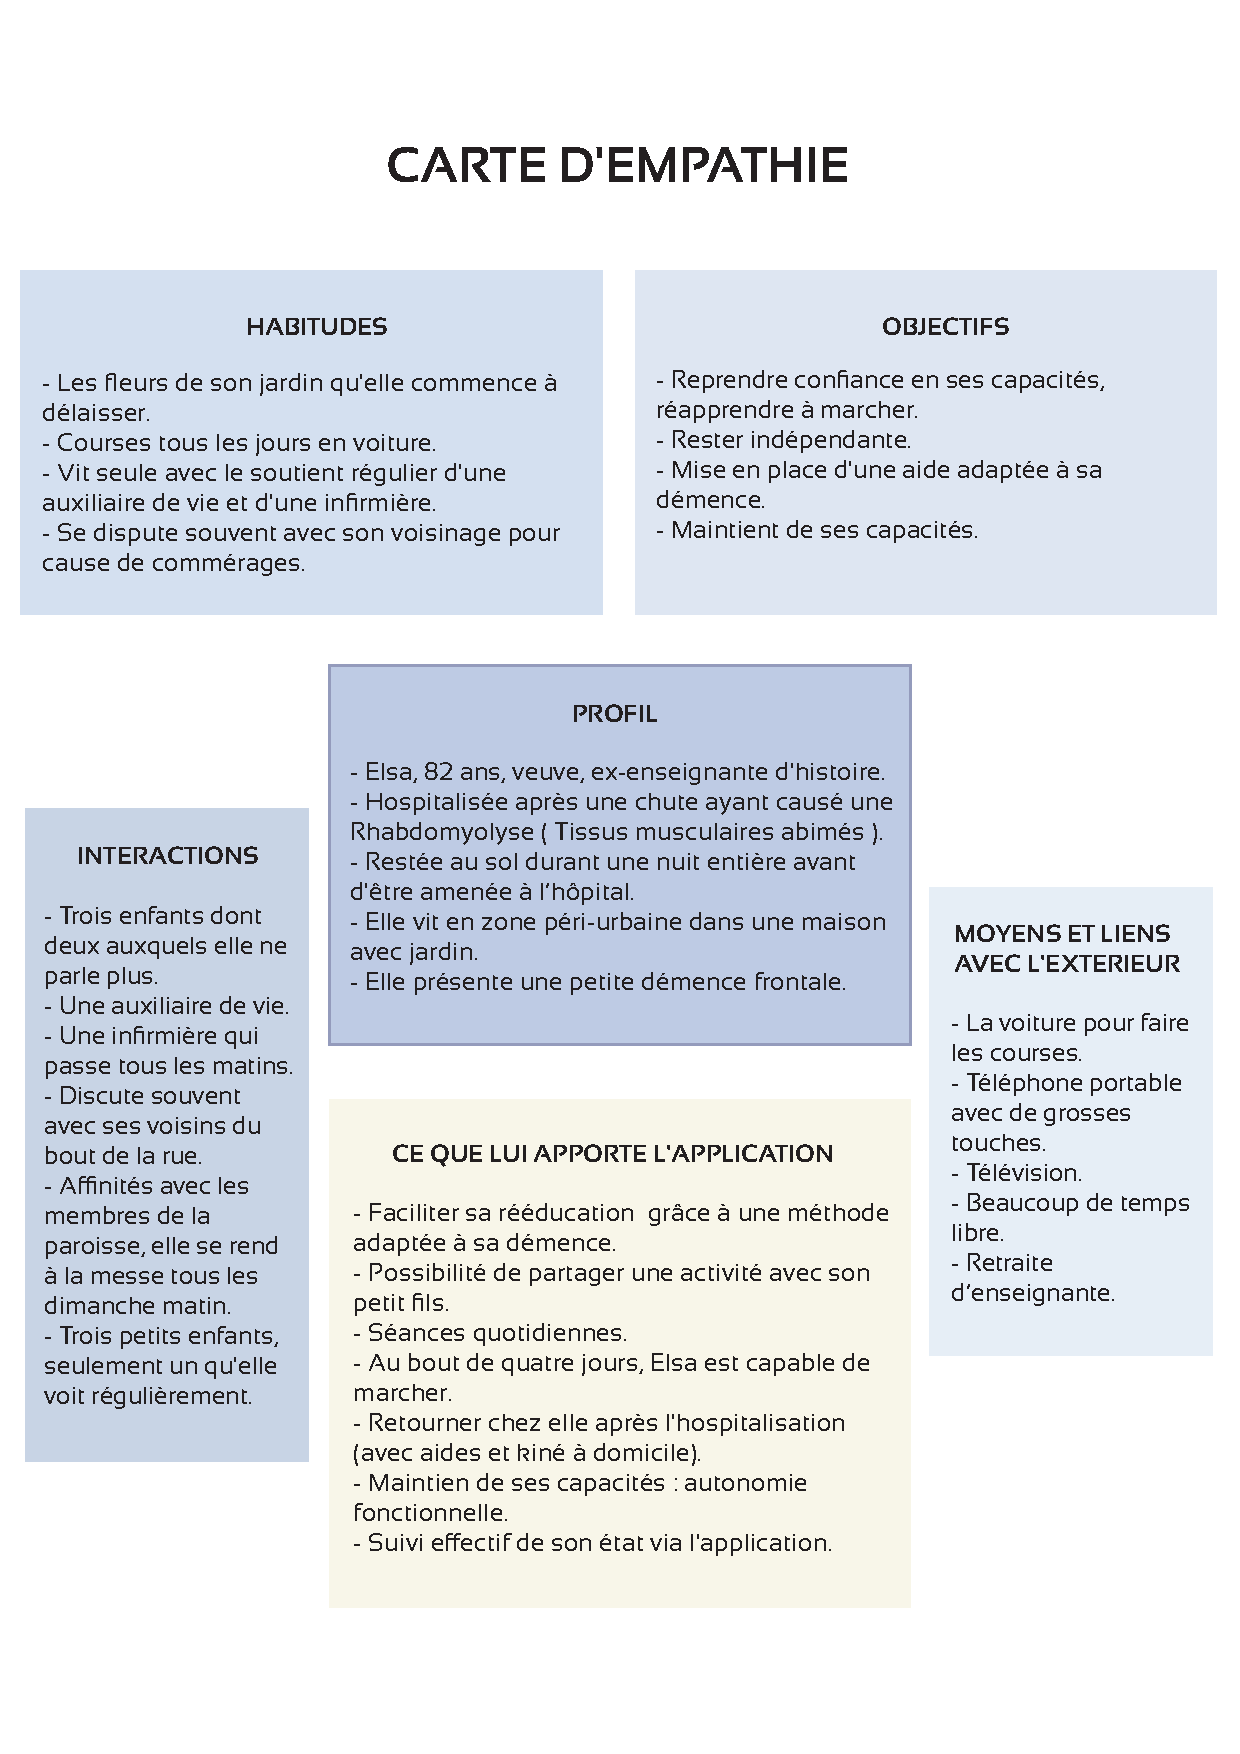
\includepdf{images/empathie_elsa}
\label{empathie_elsa}
	
	\subsubsection*{Imaginer et illustrer les cas d'utilisation}
La suite de la méthode de conception vient se servir des résultats des premières étapes. Il s'agit d'imaginer les différents cas d'utilisation de l'application. On va chercher à couvrir la totalité des fonctionnalités souhaitées de l'application dans différents contextes d'utilisation. Pour cela, on imagine des scénarios courts dans lesquels on pourra mettre en scène les utilisateurs imaginés lors de la séance de conception participative.

\paragraph{}Ces scénarios doivent comporter trois points~:
\begin{enumerate}
	\item un titre : permet de rapidement cerner la fonctionnalité ou le concept illustré.
	\item une description de la scène : elle permet de visualiser les acteurs présents, l'action en cours et les interactions.
	\item un commentaire : il s'agit d'expliquer ce qui se passe dans la scène, éventuellement comment on en est arrivé là, les objectifs en jeux ou l'intérêt de l'application ou du jeu.
\end{enumerate}

\paragraph{}Pour fournir des exemples de scénarios d'usage, je vais ici utiliser un travail issu d'un autre projet auquel j'ai participé. Il s'agissait ici de proposer une application pour aider à la rééducation de personnes lombalgiques. Le principal objectif est de faire bouger les patients~: la douleur vient de l'inactivité et reprendre une activité physique est donc indispensable. Cette séance s'est déroulée notamment en présence d'un docteur en médecine spécialisé dans la lombalgie, Arnaud Dupeyron.

\begin{quotation}
	\emph{Slide Contexte} :\\
	\textbf{Description} : Paul est dans son canapé. Un proche lui recommande de se reposer.\\
	\textbf{Commentaire} : Il a mal au dos et est en arrêt maladie pour ça. Il aimerait ne plus avoir mal. Ses proches l’encouragent à se reposer, ne pas trop bouger.
	\paragraph{}
	\emph{Slide présentation par le médecin} :\\
	\textbf{Description} : Cabinet médical, Paul est entre les mains de son médecin. Il fait des exercices devant une kinect et un ordinateur.\\
	\textbf{Commentaire} : Le nouveau médecin qui va s’occuper du dos de Paul mesure les capacités de mouvement de Paul avec notre application. Il va conseiller à Paul de se remettre à bouger. Il lui déconseille d’être sédentaire et donc, il va lui recommander d’utiliser notre application chez lui afin de l’aider à se remettre en activité.
	\paragraph{}
	\emph{Slide suivi d’un patient} :\\
	\textbf{Description} : le médecin est devant son ordinateur, il consulte le profil de Paul et visualise ses capacités.\\
	\textbf{Commentaire} : l’application présente un bilan simplifié des capacités du patient. Notre application permet un suivi du patient par le médecin en remontant des informations sur l’endurance, la souplesse, la fréquence d’utilisation, des alertes … Mais le premier but de l’application c’est de faire bouger Paul.
\end{quotation}

	
	\subsubsection*{Création de storyboards}
Les storyboards sont des organisateurs graphiques sous la forme d'illustrations ou d'images affichées dans un ordre chronologique dans le but de pré-visualiser des séquences futures. Le storyboarding est utilisé dans le développement de logiciels pour mieux identifier leurs spécifications et les différentes étapes de l'expérience de l'utilisateur.
\paragraph{}
Dans notre cas, les storyboards sont construits à partir des scénarios d'usage conçu à l'étape précédente. Elles aident les utilisateurs à comprendre comment exactement l'application doit être utilisée au moyen d'une mise en scène de ces utilisations. C'est aussi un moyen de personnaliser l'expérience et de rapprocher les futurs utilisateurs de l'application, en la rendant plus accessible.
	
	\subsubsection*{Résumé et résultats}	 
Finalement, en quelques étapes bien définies, il est possible de passer d'une simple idée partagée à la production d'un document graphique mettant en scène toutes les possibilités d'utilisation de l'application idéale répondant aux principaux objectifs que l'on s'est fixés.

\paragraph{} Cette méthode met un fort accent sur une conception collaborative de la part des différents acteurs et met l'utilisateur et les impacts au centre du processus de conception. D'un point du vue du développement, on choisira une méthodologie AGILE mettant l'accent sur des échanges réguliers entre l'équipe de développement et les utilisateurs précédemment cités, afin de vérifier que le projet reste bien en corrélation avec leurs besoins. Elle permet entre autres de partager les connaissances et les compétences des participants, ce qui contribue à la qualité globale de la conception.
 On notera par ailleurs des similarités entre la méthode proposée et les valeurs de la méthodologie AGILE, en mettant en avant la collaboration et l'adaptation ainsi que les interactions et les échanges pour se concentrer sur les objectifs de l'application.

	\subsubsection{Différences et complémentarité des solutions}
Les deux approches empruntées pour aider à la conception de jeux sérieux pour la santé sont donc bien différentes. La première cherche plutôt à définir et enregistrer des savoirs qui seront utiles dans le processus de conception. La seconde, propose une méthodologie permettant de dynamiser les échanges entre les acteurs afin de répartir les savoirs.

\paragraph{} Il n'existe actuellement pas à ma connaissance de méthode classique de conception spécifique à la création de serious games se distinguant par son efficacité. L'utilisation et la prise en compte de connaissances comme celles proposées en~\ref{part_outils}, pourraient ainsi permettre de proposer des pistes intéressantes de conception. Si ce travail était poursuivi, en travaillant spécifiquement sur chaque type de jeu ou en enrichissant la base de contrôles possibles, il serait ainsi possible d'orienter efficacement la conception de l'application.

\paragraph{} Par ailleurs les deux approches proposées sont aussi compatibles. L'intégration de savoirs, s'ils font défaut à l'équipe de conception, peut permettre d'enrichir la pensée et les solutions envisagées. C'est aussi une manière d'envisager d'autres approches, comme utiliser le contrôle comme lien entre les composantes médicales et ludiques. La méthode de conception participative présentée peut trouver sa place dans le processus de conception avant l'utilisation de l'ensemble des outils. Ceux-ci pourront être plus justement utilisés lors de la phase de développement du l'application, en compléments des documents produits pendant la conception participative.	

%		\subsubsection{}
%	
%	-travail avec les thérapeutes
%	-répondre aux objectifs thérapeutique par un gamedesign
%		- hammer \& Planks et l'équilibre (voir rapport d'anais)
%	-ajustement de la difficulté et lien avec la thérapie : impact des paramètres en terme de difficulté (équilibre et dos?)
